%"###############################################
%
% Classification supervisée
%
%###############################################

% VPPBS: prévision du profil de guérison
%
%###############################################

\subsubsection{VPPBS: prévision du profil de guérison}

Comme pour les exercices précédents, nous évaluons l'efficacité des embranchements de l'arbre de régression complet. La figure~\ref{fig-vppbs-regtree-optim-healing-class} montre un point d'inflexion pour cp=0,13. L'arbre élagué sur ce critère, est représenté figure~\ref{fig-vppbs-regtree-ipss12}.

\begin{figure}[H]
\centering
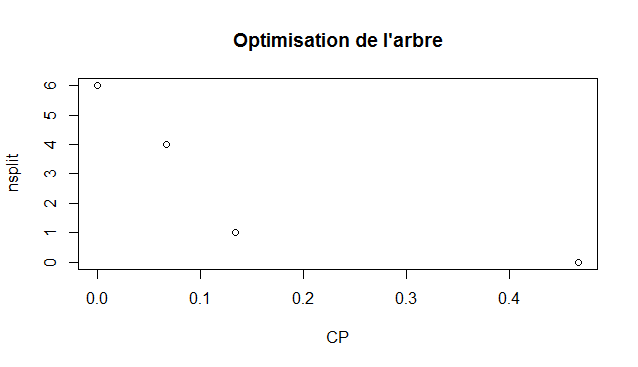
\includegraphics[width=0.75\textwidth]{../Fig/VPPBS/vppbs-regtree-optim-healing-class.png}
\caption{VPPBS: Optimisation de l'arbre de régression pour profil de guérison}
\label{fig-vppbs-regtree-optim-healing-class}
\end{figure}

\subsubsection{VPPBS: prévision du profil de guérison}
\begin{figure}[H]
\centering
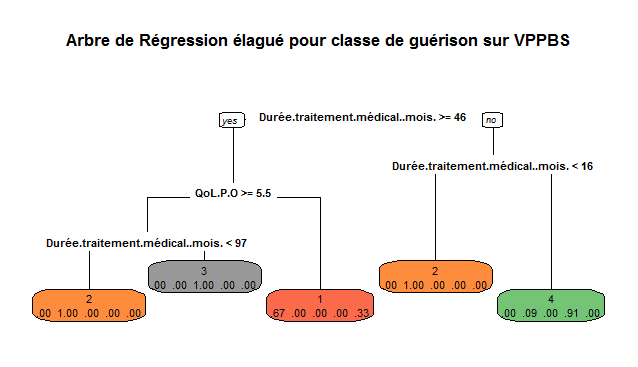
\includegraphics[width=0.75\textwidth]{../Fig/VPPBS/vppbs-regtree-healing-class.png}
\caption{VPPBS: Arbre de régression pour profil de guérison}
\label{fig-vppbs-regtree-ipss12}
\end{figure}

En appliquant l'arbre de régression sur l'échantillon de validation, nous obtenons des prévisions soit plutôt sûres (probabilités très fortes pour 3 patients sur 7), soit mitigées, comme illustré figure~\ref{fig-vppbs-predict-healing-class}.

\begin{figure}[H]
\centering
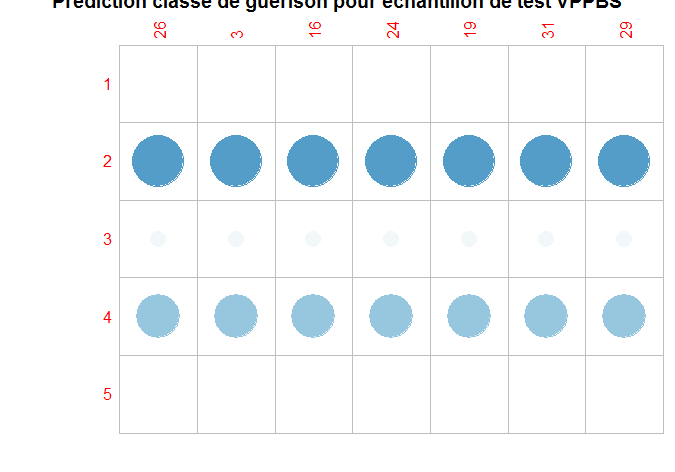
\includegraphics[width=0.75\textwidth]{../Fig/VPPBS/vppbs-predict-healing-class.png}
\caption{VPPBS: Prédiction du profil de guérison}
\label{fig-vppbs-regtree-predict-ipss12}
\end{figure}

\begin{lstlisting}[language=R]
> table(validation = testVPPBSclass$postVPPBS_class, prediction =  predict(dt, testVPPBSclass, type="class"))
          prediction
validation 1 2 3 4 5
         1 1 0 0 0 0
         2 0 0 0 1 0
         3 0 0 1 0 0
         4 0 0 0 1 0
         5 3 0 0 0 0
\end{lstlisting}
Soit un taux d'erreur de 57\%.

Par contre, en utilisant une forêt aléatoire construite sur l'ensemble d'apprentissage, nous constatons alors, ci-dessous, un taux d'erreur de 0\%. La classification des profils pré-opératoires, s'avère donc fiable pour recommander une indication d'opération VPPBS et le profil de guérison associé.

\begin{lstlisting}[language=R]
> table(validation = testVPPBSclass$postVPPBS_class, prediction =  predict(rf, testVPPBSclass))
          prediction
validation 1 2 3 4 5
         1 1 0 0 0 0
         2 0 1 0 0 0
         3 0 0 1 0 0
         4 0 0 0 1 0
         5 0 0 0 0 3
\end{lstlisting}

